\documentclass{article}

\usepackage{indentfirst}
\usepackage{color}
\usepackage{graphicx}
\usepackage{amsmath}
\usepackage{epsfig}
\usepackage{geometry}
\usepackage{setspace}
\usepackage{xcolor}
\usepackage{listings}

\lstset{%
alsolanguage=Python,
% language={[Visual]Python},       %language为,还有{[Visual]Python}
%alsolanguage=[ANSI]C,      %可以添加很多个alsolanguage,如alsolanguage=matlab,alsolanguage=VHDL等
%alsolanguage= tcl,
alsolanguage= XML,
tabsize=4, %
  frame=shadowbox, %把代码用带有阴影的框圈起来
  commentstyle=\color{red!50!green!50!blue!50},%浅灰色的注释
  rulesepcolor=\color{red!20!green!20!blue!20},%代码块边框为淡青色
  keywordstyle=\color{blue!90}\bfseries, %代码关键字的颜色为蓝色,粗体
  showstringspaces=false,%不显示代码字符串中间的空格标记
  stringstyle=\ttfamily, % 代码字符串的特殊格式
  keepspaces=true, %
  breakindent=22pt, %
  numbers=left,%左侧显示行号 往左靠,还可以为right,或none,即不加行号
  stepnumber=1,%若设置为2,则显示行号为1,3,5,即stepnumber为公差,默认stepnumber=1
  %numberstyle=\tiny, %行号字体用小号
  numberstyle={\color[RGB]{0,192,192}\tiny} ,%设置行号的大小,大小有tiny,scriptsize,footnotesize,small,normalsize,large等
  numbersep=8pt,  %设置行号与代码的距离,默认是5pt
  basicstyle=\footnotesize, % 这句设置代码的大小
  showspaces=false, %
  flexiblecolumns=true, %
  breaklines=true, %对过长的代码自动换行
  breakautoindent=true,%
  breakindent=4em, %
  escapebegin=\begin{CJK*}{GBK}{hei},escapeend=\end{CJK*},
  aboveskip=1em, %代码块边框
  tabsize=2,
  showstringspaces=false, %不显示字符串中的空格
  backgroundcolor=\color[RGB]{245,245,244},   %代码背景色
  %backgroundcolor=\color[rgb]{0.91,0.91,0.91}    %添加背景色
  escapeinside=``,  %在``里显示中文
  %% added by http://bbs.ctex.org/viewthread.php?tid=53451
  fontadjust,
  captionpos=t,
  framextopmargin=2pt,framexbottommargin=2pt,abovecaptionskip=-3pt,belowcaptionskip=3pt,
  xleftmargin=4em,xrightmargin=4em, % 设定listing左右的空白
  texcl=true,
  % 设定中文冲突,断行,列模式,数学环境输入,listing数字的样式
  extendedchars=false,columns=flexible,mathescape=true
  % numbersep=-1em
}

\geometry{left=2.54cm,right=2.54cm,top=2.54cm,bottom=2.54cm}
\begin{document}
\begin{spacing}{1.2}
\vspace*{0.25cm}

\thispagestyle{empty}

\begin{center}
\hrulefill

\thispagestyle{empty}


\begin{large}
\sc{CompSci 261P \\ Data Structures}
\end{large}

\hrulefill

\vspace*{5cm}
\begin{Large}
\sc{{Project 1: Hashing algorithms}}
\end{Large}

\vspace{2em}

\end{center}


\vfill

\begin{table}[h!]
\flushleft
\begin{tabular}{lll}
Name: Xingyou Ji \hspace*{2em}
\\
Date: 23 October 2019

\end{tabular}
\end{table}

\hfill

\newpage
\tableofcontents

\newpage
\section{Hash Chaining}
\subsection{Construction}
In the method of hash chaining, each cell of the hash table is a linked list, with each ListNode storing a pair of key-value. Therefore, in order to implement the hash algorithm, I first implement a linked list.
The supported functions and corresponding implementations as well as the amortized time are shown below.

\subsubsection{Linked List Construction}
For a ListNode, it has two members: a key-value pair and a pointer pointing to the next node.

The running time for creation is in $O(1)$. 
\begin{lstlisting}[language=Python]
from kv import *
class ListNode(object):
    def __init__(self, k, v):
        self.kv = KVPair(k, v)
        self.next = None
\end{lstlisting}

\subsubsection{Linked List Search}
To perform a search operation in a linked list, we have to traverse the whole linked list from the head node until a match is found.

The running time is in $O(n)$, where $n$ denotes the length of the linked list.
\begin{lstlisting}[language=Python]
def search(self, key):
    dummy = ListNode(-1, -1)
    curr = dummy
    curr.next = self.head
    while curr.next:
        if curr.next.kv.key == key:
            return curr.next.kv.val
        else:
            curr = curr.next
    return -1
\end{lstlisting}

\subsubsection{Linked List Insert}
There could be two situations when performing  an insert operation. If the key exists in the linked list, then we should update its corresponding value. Otherwise, insert a new ListNode to the end.

The running time of insert is in $O(n)$, as we need to traverse the whole linked list.
\begin{lstlisting}[language=Python]
def insert(self, key, val):
    dummy = ListNode(-1, -1)
    curr = dummy
    curr.next = self.head
    isExisted = False
    while curr.next:
        if curr.next.kv.key == key:
            curr.next.kv.val = val
            isExisted = True
            break
        else:
            curr = curr.next
    if not isExisted:
        node = ListNode(key, val)
        curr.next = node
    self.head = dummy.next
    return dummy.next
\end{lstlisting}

\subsubsection{Linked List Remove}
To perform a remove operation, we have to traverse the whole linked list, thus causing the running time in $O(n)$.
\begin{lstlisting}[language=Python]
def remove(self, key):
    dummy = ListNode(-1, -1)
    curr = dummy
    curr.next = self.head
    while curr.next:
        if curr.next.kv.key == key:
            curr.next = curr.next.next
            break
        else:
            curr = curr.next
    self.head = dummy.next
    return dummy.next
\end{lstlisting}

\subsubsection{Structures of Hash Chaining}
Since the linked list is done, we can define our hash chaining in the following structure.
\begin{lstlisting}[language=Python]
class Chaining(object):
    def __init__(self):
        self.N = 373
        self.alpha = 0
        self.cnt = 0
        self.table = [LinkList() for i in range(self.N)]
\end{lstlisting}

\subsection{Hash Functions}
For the hashing chaining, I choose the hash function to be 
\begin{equation*}
    h(k) = k \bmod N
\end{equation*}

The reason for doing so is to separate data as uniformly as possible and make sure that for a randomly generated key-val pair, it has the same likelihood to fall into each cell. So, theoretically, situations would not happen where some cell contains a linked list that is much longer than others.

\subsection{Supported Functions}
\subsubsection{Search}
The idea of search is to first calculate the hash value of key, and use linked list search to check whether the key-value pair exists.

The running time of search is in $O(1 + Len(H(k)))$.
\begin{lstlisting}[language=Python]
def search(self, key):
    k = self.hash(key)
    return self.table[k].search(key)
\end{lstlisting}

\subsubsection{Insert}
The idea is to first locate the cell, and do a linked list insert operation.

The running time of insert is in $O(1 + Len(H(k)))$.

Notice that if too many elements have been added to the hash table, it is likely to have collisions, thus lowering the running speed. To avoid this case, we can calculate the load factor $\alpha$ when doing insert, and choose to do rehashing accordingly. 
It is common and proved to be efficient to limit $\alpha$ within the range $[\frac{1}{4}, \frac{3}{4}]$. This feature is supported in the codes I submit in the zip file, and I would omit the description here to avoid being too tedious.
\begin{lstlisting}[language=Python]
def insert(self, key, val):
    k = self.hash(key)
    isExisted = (self.table[k].search(key) != -1)
    self.table[k].insert(key, val)
    if not isExisted:
        self.cnt += 1
        self.alpha = self.cnt / self.N
        if self.alpha >= 1:
            self.N *= 2
            self.rehash()
\end{lstlisting}

\subsubsection{Remove}
The idea is to first locate the cell, and do a linked list insert operation.

The running time of remove is in $O(1 + Len(H(k)))$.
\begin{lstlisting}[language=Python]
def remove(self, key):
    k = self.hash(key)
    isExisted = (self.table[k].search(key) != -1)
    self.table[k].remove(key)
    if not isExisted:
        self.cnt -= 1
        self.alpha = self.cnt / self.N
        if self.alpha <= 0.25:
            self.N /= 2
            self.rehash()
\end{lstlisting}

\subsubsection{Rehash}
When doing insert or remove operation, it is possible that the load factor becomes too large or too small. A large load factor indicates that there will be many collisions and a small load factor indicates that the space efficiency is low. Therefore, in this case, we need to do a rehash, namely, when $\alpha \leq 0.25$ or $\alpha \geq 0.75$.

The running time is in $O(N\cdot\max(Len(H(k))))$.
\begin{lstlisting}[language=Python]
def rehash(self):
    all = []
    self.cnt = 0
    for lst in self.table:
        head = lst.head
        while head:
            kv = head.kv
            all.append(kv)
            head = head.next
    self.table = [LinkList() for i in range(0, self.N)]
    for kv in all:
        self.insert(kv.key, kv.val)
\end{lstlisting}

\subsection{Theoretical Analysis}
For hash chaining, each operation will cost a total time in $O(1 + Len(H(k)))$.

To formulate, for a pair p, the expected running time is:
\begin{align*}
    E[\text{time/operation}] &= O(1 + E[Len(H(k))])\\
    &= O(1 + \Sigma_{q \in S - p}(H(q.k) == H(p.k)))\\
    &= O(1 + \frac{n-1}{N})\\
    &= O(1 + \alpha)
\end{align*}

\subsection{Test Cases}
\subsubsection{Generate Procedure}
I wrote a generate\_testcase function in main.py, which can randomly generate numbers in the range within 0 and 100 to act as the parameter key and val. I make the load factor in the range of $0.05$ to $0.95$ with step length of $0.05$, and calculate the corresponding number of records the input should contain.

Once the test cases for one particular $\alpha$ are generated, I stored these records into the file that is dynamically generated, so that I can read these records and make sure these records will not change when I test the hashing algorithm. This is very important since when doing the performance test, we want to make sure that all outer environment is fully identical.

\subsubsection{Correctness Test}
When checking for correctness, I first generated 20 operations of insert to store 20 pairs in the hash table.

Then, I did 20 search operations. Within them, some search for non-existed pairs.

Last, I did 10 remove operations. Within them, some remove non-existed pairs, and it will cause no effect.

So far, I have tested the functionality of hash chaining algorithm. But, more efforts should still be put on corner cases, which is repeated pairs and non-existed pairs.

Therefore, I randomly generated a testcase containing 70 operations including Search, insert and remove, each type containing multiple corner cases. All the tests are passed, indicating that there is no error inside the supported functions.

\subsubsection{Efficiency Test}
The load factor $\alpha$ is chosen from $0.05$ to $0.95$ with step length of $0.05$. Therefore, a total of $19$ records can be obtained, and that will be sufficient to obtain a linear relationship in the log-log plot.

In practice, I generate test cases each containing $(\alpha\cdot N)$ key-value pairs, and do the insert operation. The randomly generated test cases will be normally distributed on each cell. Therefore, there will not be too many or too few collisions, and the result obtained will be very similar to the theoretical case. 

After running tests, I collect $\alpha$ and running time to have a log-log plot. The reason of using log-log scale is that if we can find a linear relationship in a log-log plot, then it is very convenient to transform into a polynomial relationship. In normal sense, a polynomial relationship means high efficiency.

You can view the test cases in project/testcase/insert/. The test result is shown below.

In the efficiency test, I used the actual clock time. The reason for doing so is that when doing the performance test, actual clock time reflects the real situation of an algorithm. The running time is not only about the number of cells encountered, but also is related to the data structures. Therefore, it is more practical to use the clock time as the measure.

When I obtain the test result, I compare it with amortized time rather than the worst case time. The reason for doing so is that when analyzing the performance of an algorithm, we would try to avoid the occurrence of worst case, and we put more emphasis on average performance. For example, the worst case happens when there are a huge number of collisions. However, this issue is fixed in the codes by doing rehash.  
\begin{itemize}
    \item Insert\\
    Using the original data without applying a log log trick, the plot is shown below in Fig \ref{chain-origin}.
    \begin{figure}[!htb]
        \centering
        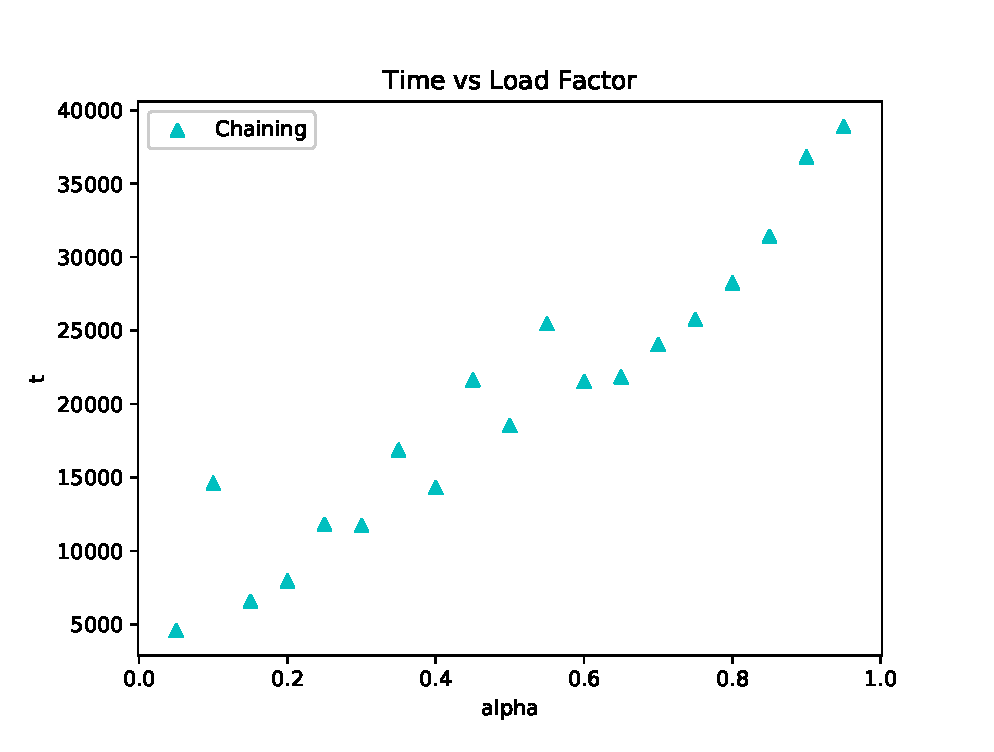
\includegraphics[width=0.6\textwidth]{../output/fig/insert_original_chain.eps}
        \caption{Hashing chaining (Insert).}
        \label{chain-origin}
    \end{figure}

    However, limited information can be obtained from Fig \ref{chain-origin}.

    In order to have a linear relation, the x-axis is chosen to be $\log(\alpha)$ and the y-axis is chosen to be $\log(T)$, and the linear fitting is shown in Fig \ref{chain-insert}.
    \begin{figure}[!htb]
        \centering
        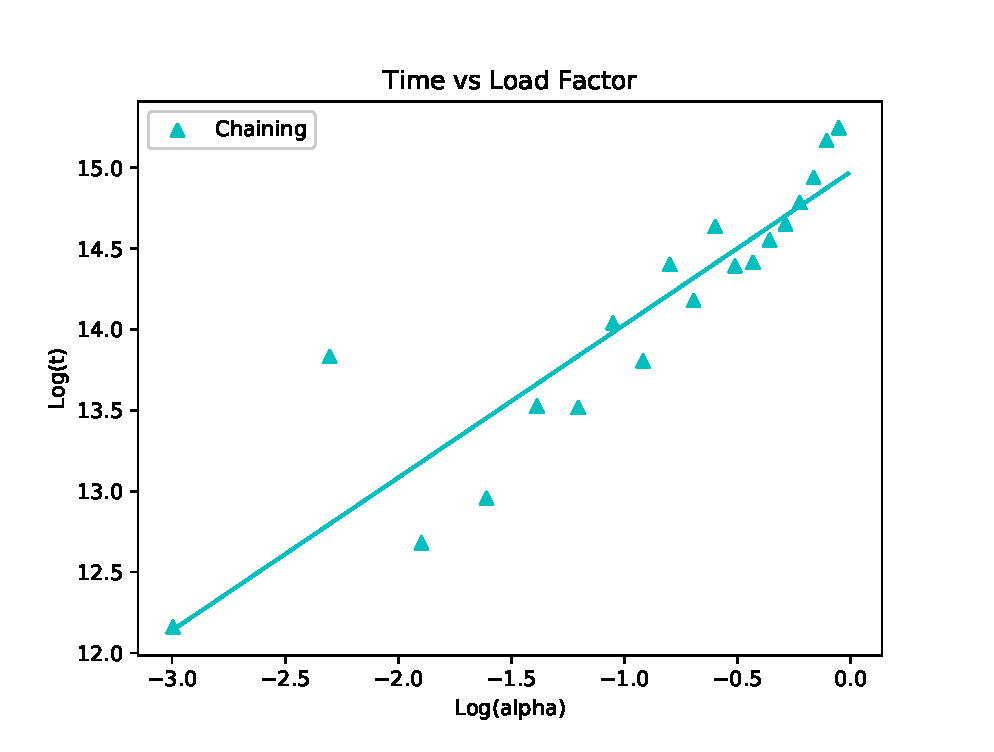
\includegraphics[width=0.6\textwidth]{../output/fig/insert_chain.eps}
        \caption{Log-log plot for hashing chaining (Insert).}
        \label{chain-insert}
    \end{figure}

    I use the scipy.optimize.curve\_fit function in Python, and the result is:
    \begin{equation*}
        \log(T) = 0.945 \cdot \log(\alpha) + 14.974
    \end{equation*}
    which can be further simplify to polynomial form:
    \begin{equation*}
        T = \alpha^{0.945}\cdot 2^{14.974}
    \end{equation*}

    Recall that the expected running time is in $O(1+\alpha)$, which is a first order polynomial of $\alpha$, the result is close and thus makes sense.
\end{itemize}

\section{Cuckoo Hashing}
\subsection{Construction}
\subsubsection{Structures of Cuckoo Hashing}
For a cuckoo hashing, it contains two hash tables and two hash functions. In order to prevent infinite loops, I set a limit to detect whether the cuckoo hashing requires rehash.

The structures of the cuckoo hashing class is shown below.
\begin{lstlisting}[language=Python]
class Cuckoo(object):
    def __init__(self):
        self.N = 373
        self.alpha = 0
        self.limit = 300
        self.pos = [nan for i in range(0, 2)]
        self.table = [[KVPair(nan, nan) for i in range(0, self.N)], [KVPair(nan, nan) for j in range(0, self.N)]]
    def hash(self, func, key):
        if func == 1:
            return key % self.N
        elif func == 2:
            return floor(key / self.N) % self.N
\end{lstlisting}

\subsection{Hash Functions}
For cuckoo hashing, there are two hash tables inside. I choose the two hash functions to
\begin{align*}
    h_1(k) &= k\bmod N\\
    h_2(k) &= (k / N) \bmod N
\end{align*}

The reason for choosing the first hash function is to separate data as uniformly as possible so that for a randomly generated testcase, it has equal likelihood to be mapped into each cell. Otherwise, situations may happen where some cells are much more likelihood to be mapped to than others. In this case, lots of evictions have to be done, thus reducing the efficiency of the algorithm.

The reason for choosing the second hash function is similar. My idea is to first convert the key into another value, and apply the same priniple as the first hash function.

\subsection{Supported Functions}
\subsubsection{Search}
When performing a search operation, we need to check two places in two hash tables.

The running time is in $O(1)$.
\begin{lstlisting}[language=Python]
def search(self, key):
    for i in range(0, 2):
        k = self.hash(i + 1, key)
        if self.table[i][k].key == key:
            return self.table[i][k].val
\end{lstlisting}

\subsubsection{Insert}
The insert operation in cuckoo hashing is quite different from other hashing methods.

First, we do a search in the two tables to see whether we only need to do an update. If so, update the corresponding value and return.

If the pair to insert is new, then we have to check whether its corresponding position in table 1 is availbale. If so, put the new pair there and return.

If not, put the new pair in its corresponding position in table 1, and do a insert operation for the pair which was in that cell originally. The insert operation for this pair starts to check table two. It is a recursive process, and during each step, we update the counter. Once the counter reaches the limit, it means there is an infinite loop and return.

Since the insert operation only requires to check certain cell in two hash tables, the running time is in $O(1)$.
\begin{lstlisting}[language=Python]
def helper(self, key, val, table_id, cnt):
    if cnt == self.limit:
        self.N *= 2
        self.rehash()
    for i in range(0, 2):
        self.pos[i] = self.hash(i + 1, key)
        if self.table[i][self.pos[i]].key == key:
            self.table[i][self.pos[i]].val = val
            return
    if self.table[table_id][self.pos[table_id]].key is not nan and self.table[table_id][self.pos[table_id]].val is not nan:
        kv = self.table[table_id][self.pos[table_id]]
        self.table[table_id][self.pos[table_id]] = KVPair(key, val)
        self.helper(kv.key, kv.val, (table_id + 1) % 2, cnt + 1)
    else:
        self.table[table_id][self.pos[table_id]] = KVPair(key, val)

def insert(self, key, val):
    self.helper(key, val, 0, 0)
\end{lstlisting}

\subsubsection{Remove}
The idea of remove is to check two hash tables in order whether the target cell has a pair. If so, remove the pair. In my code implementation, it is to make the cell return to its initial state. 

Since it only requires to look up in two hash tables, the running time is in $O(1)$.
\begin{lstlisting}[language=Python]
def remove(self, key):
    for i in range(0, 2):
        k = self.hash(i + 1, key)
        if self.table[i][k].key == key:
            self.table[i][k] = KVPair(nan, nan)
\end{lstlisting}

\subsubsection{Rehash}
In the insert function, if we reach the limit of search, it indicates that there are too many collisions now, and we should do a rehash.

The basic idea is to twice the cell number and insert all the elements again. The running time is in $O(N)$.
\begin{lstlisting}[language=Python]
def rehash(self):
    all = []
    for i in range(0, 2):
        for kv in self.table[i]:
            if kv.key is not nan and kv.val is not nan:
                all.append(kv)
    self.table = [[KVPair(nan, nan) for i in range(0, self.N)], [KVPair(nan, nan) for i in range(0, self.N)]]
    for kv in all:
        self.insert(kv.key, kv.val)
\end{lstlisting}

\subsection{Theoretical Analysis}
For an arbitrary sequence of operations, it could contain multiple search, insert and remove. As I have included in the previous section, search, insert and remove all have $O(1)$ running time since the basic idea is to look up certain cells in two hash tables.

Suppose a sequence contains $n$ operations, based on the previous analysis, the total running time of cuckoo hashing is in $O(n)$.

Recall the definition of load factor $\alpha:=\frac{n}{N}$, hence $n=\alpha N$. Therefore, the running time can be rewritten as $O(\alpha N)$.
\subsection{Test Cases}
\subsubsection{Generate Procedure}
I read the files that is generated in the hash chaining, and do the following test.

\subsubsection{Correctness Test}
When checking for correctness, I first generated 50 operations of insert to store 50 pairs in the two hash tables.

Then, I did 25 search operations. Within them, some search for non-existed pairs.

Last, I did 25 remove operations. Within them, some remove non-existed pairs, and it will cause no effect.

So far, I have tested the functionality of cuckoo hashing algorithm. I still need to test corner cases, which is repeated pairs and non-existed pairs.

Therefore, I randomly generated a testcase containing 70 operations including search, insert and remove, each type containing multiple corner cases. All the tests are passed, indicating that there is no error inside the supported functions.

\subsubsection{Efficiency Test}
In the efficiency test, I used the actual clock time. The reason for doing so is that when doing the performance test, actual clock time reflects the real situation of an algorithm. The running time is not only about the number of cells encountered, but also is related to the data structures. Therefore, it is more practical to use the clock time as the measure.

The reason of choosing actual clock time and amortized time is explained in section 1.5.3.
\begin{itemize}
    \item Insert\\
    Using the original data without applying a log log trick, the plot is shown below in Fig \ref{chain-origin}.
    \begin{figure}[!htb]
        \centering
        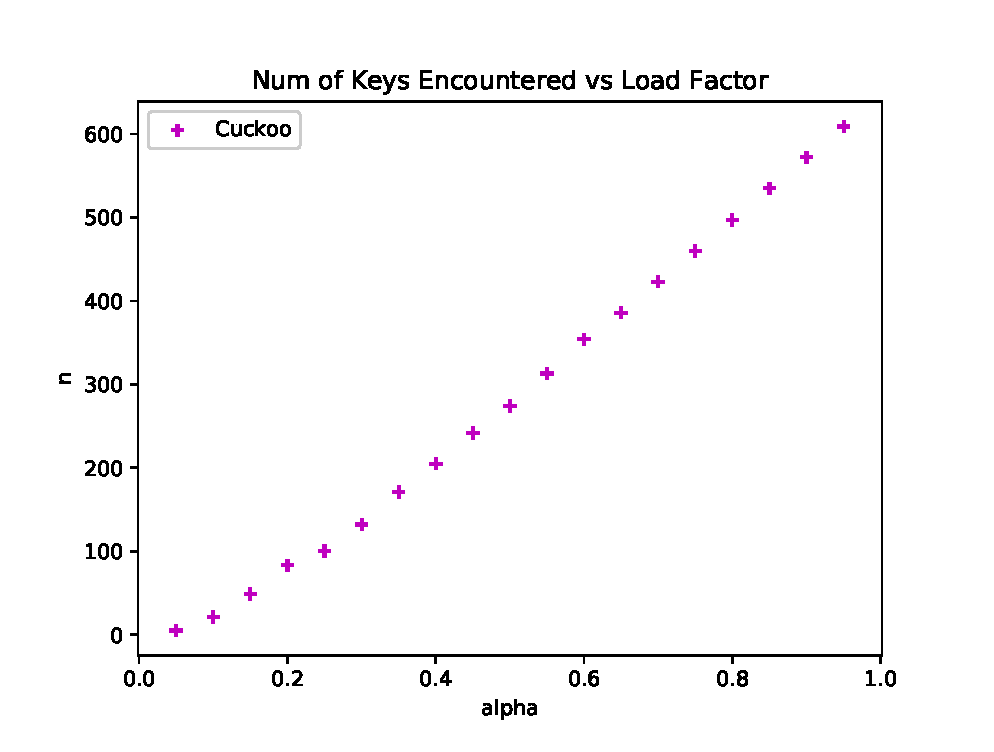
\includegraphics[width=0.6\textwidth]{../output/fig/insert_original_cuckoo.eps}
        \caption{Cuckoo hashing (Insert).}
        \label{cuckoo-origin}
    \end{figure}

    However, limited information can be obtained from Fig \ref{cuckoo-origin}.

    In order to have a linear relation, the x-axis is chosen to be $\log(\alpha)$ and the y-axis is chosen to be $\log(T)$. I use the scipy.optimize.curve\_fit in Python to get the linear fitting as shown in Fig \ref{cuckoo-insert}. The result is:
    \begin{figure}[!htb]
        \centering
        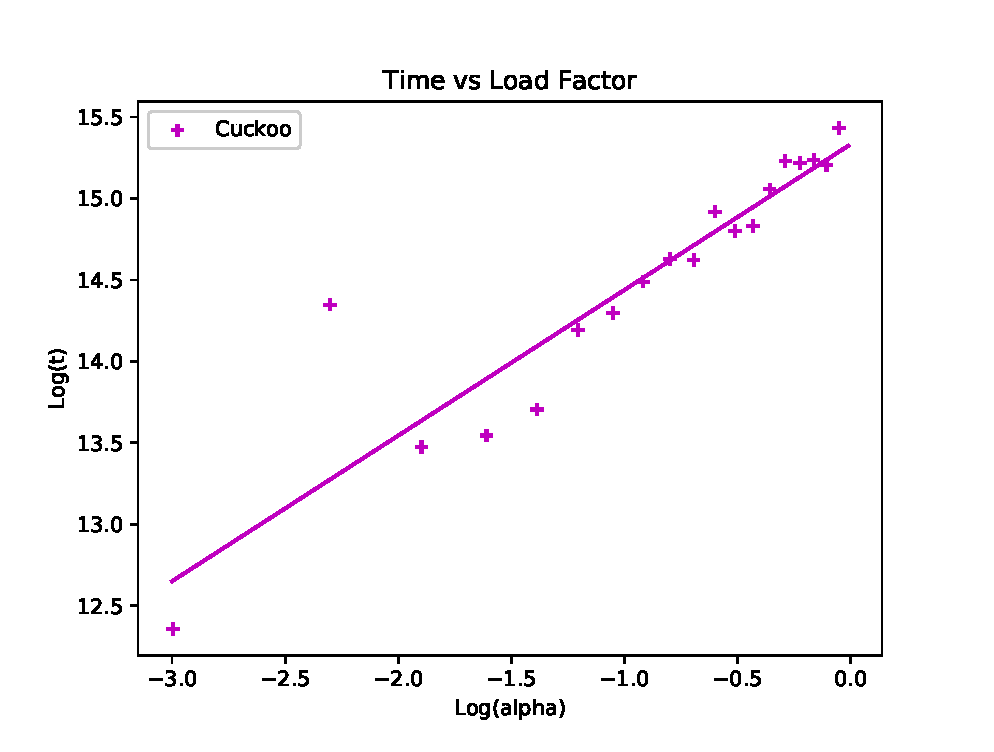
\includegraphics[width=0.6\textwidth]{../output/fig/insert_cuckoo.eps}
        \caption{Log-log plot for cuckoo hashing (Insert).}
        \label{cuckoo-insert}
    \end{figure}
    
    \begin{equation*}
        \log(T) = 0.894 \cdot \log(\alpha) + 15.332
    \end{equation*}
    which can be further simplify to polynomial form:
    \begin{equation*}
        T = \alpha^{0.894}\cdot 2^{15.332}
    \end{equation*}
    
    Recall that the expected running time is in $O(\alpha N)$, which is a first order polynomial of $\alpha$, the result is close and thus makes sense.
\end{itemize}

\end{spacing}
\end{document}